\documentclass[a4paper,12pt, twoside]{article}
%\documentclass[a4paper,12pt, twoside]{book}

\usepackage[papersize={210mm,297mm},tmargin=20mm,bmargin=20mm,lmargin=20mm,rmargin=20mm]{geometry}

\usepackage[utf8]{inputenc}
%https://mirror.hmc.edu/ctan/macros/latex/contrib/babel-contrib/turkish/turkish.pdf
\usepackage[english]{babel}
%\usepackage[T1]{fontenc}

\usepackage{amsmath,amssymb,mathabx}%\for eqref
\usepackage{lscape}

\usepackage{hyperref}
\hypersetup{
    colorlinks,
    citecolor=black,
    filecolor=black,
    linkcolor=blue,
    urlcolor=red}
  

%%% \usepackage{svg}
%%% https://tex.stackexchange.com/questions/122871/include-svg-images-with-the-svg-package/129854
\usepackage{graphicx}
\graphicspath{ {./figurler/} }

\usepackage[colorinlistoftodos]{todonotes}
\usepackage{fancyhdr}

\usepackage{indentfirst}
%% paragraf girintisi
\setlength{\parindent}{5ex}

%% Daha sonra yazılacak kısımları not düşmek için...
\newcommand{\YAZILACAK}{{\vspace{18pt}\bf\Large \color{red} YAZILACAK}}


\pagestyle{fancy}
\fancyhf{}
\lhead{ Kuantum Fiziği }
\chead{\thepage}
\rhead{Mesut Karakoç}
\lfoot{Akdeniz Üniversitesi}
\cfoot{}
%\rfoot{BF}

\title{Akdeniz Üniversitesi\\ Fen Fakültesi - Fizik Bölümü\\FİZ319 Kuantum Fiziği Ders Notları}

\author{\setlength{\unitlength}{6mm}
\begin{picture}(10,10)
\put(1.1,0){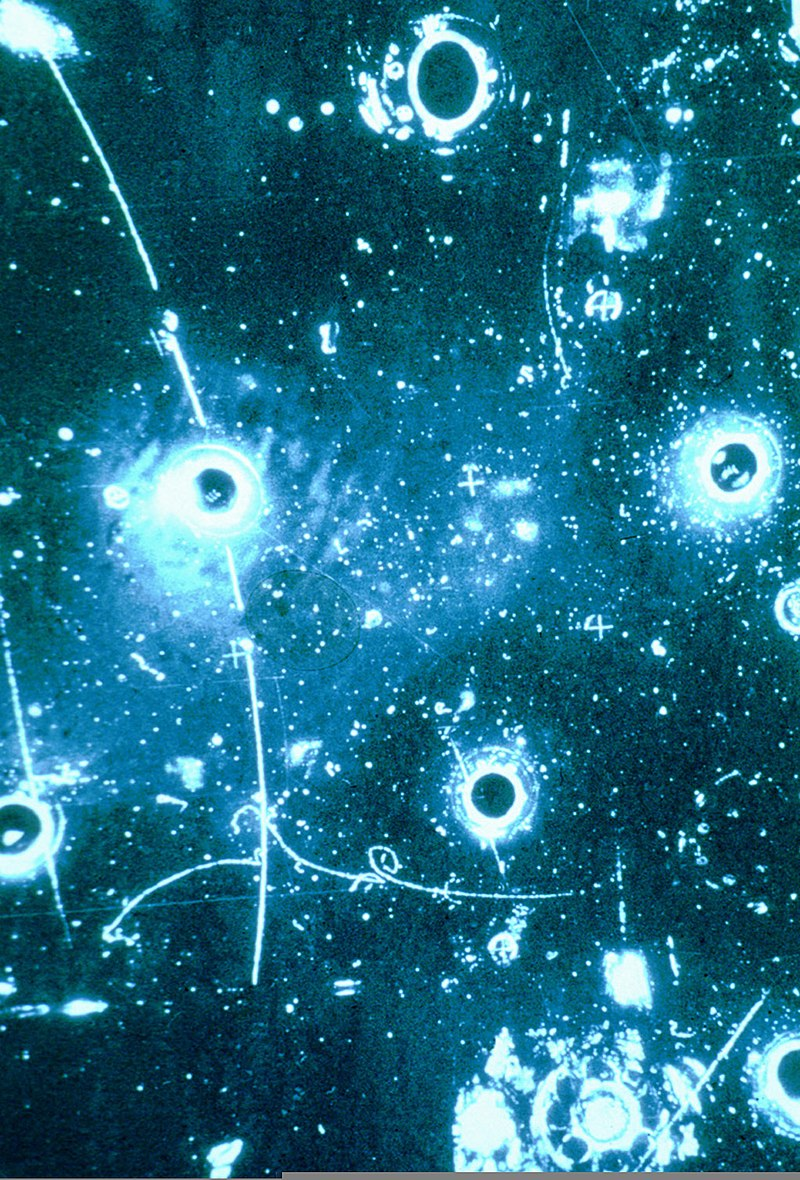
\includegraphics[width=4.5cm]{Leptonic_event_in_Gargamelle_bubble_chamber.jpg}}
\end{picture} \\ Doç. Dr. Mesut Karakoç}


\date{\today}

\begin{document}

%% Turkish babel problem
%% https://tex.stackexchange.com/questions/160385/newgeometry-doesnt-work-with-turkish-babel-package
%%\shorthandoff{=}% Make = not active any more

\maketitle

\newpage

% change name to "İçindekiler"
\renewcommand{\contentsname}{İçindekiler}
\tableofcontents{}

\listoffigures
 
\listoftables

\newpage

{
\hspace{.5\textwidth}
\begin{minipage}{.5\textwidth}
\raggedleft
If all this damned quantum jumps were really to stay, I should be
sorry I ever got involved with quantum theory.

—Erwin Schrödinger
\cite{book:Ficek}

%% Latince için
%% post iacturam quis non sapit!
%% Who is not wise after he has lost something?
%% https://quizlet.com/23756827/latin-proverbs-h-flash-cards/
\end{minipage}
}

\setcounter{section}{2} %% THIS WILL BE DELETED when all chapters merged!
\section{Schrödinger Denkleminin Ayrıştırılması, Özdeğerleri ve Özfonksiyonları}

Bu bölümde bir parçacığın veya sistemin etkisinde olduğu potansiyelin $V(x)$ zamandan bağımsız olması halinde, Schrödinger denkleminin sadece konum ve sadece zaman değişkenlerini içeren iki çiftlenmiş denklem seti halinde yazılabileceğini göreceğiz. Sadece konum değişkenine bağlı olarak yazılan yeni denklemi zamandan bağımsız Schrödinger denklemi olarak adlandırıyoruz. Devamında zamandan bağımsız denklem için özdeğer, özfonksiyon kavramlarını tartışacağız ve bazı potansiyeller için bu denklemin çözümlerini inceleyeceğiz. 

\subsection{Zamandan Bağımsız Schrödinger Denklemi}
%%
Bir önceki bölümde elde ettiğimiz zamana bağlı Schrödinger denklemini \emph{Hamilton} işlemcisini kullanarak,
%%
\begin{equation}
\hat H \psi ( x , t ) = i \hbar \frac { \partial \psi ( x , t ) } { \partial t }
\label{eq:time_depended_schrodinger_eq_op_form}
\end{equation}
%%
şeklinde yazabileceğimizi ve dalga fonksiyonlarıyla açık halini de, 
%%
\begin{equation}
- \frac { \hbar ^ { 2 } } { 2 m } \frac { \partial ^ { 2 } \psi ( x , t ) } { \partial x ^ { 2 } } + V ( x ) \psi ( x , t ) = i \hbar \frac { \partial \psi ( x , t ) } { \partial t }
\label{eq:time_depended_schrodinger_eq}
\end{equation}
%%
şeklinde yazabileceğimizi görmüştük.  Yukarıda tekrar yazdığımız zamana bağlı Schrödinger denklemi  bir kısmi diferansiyel denklemdir.  Kısmi diferansiyel denklemlerin birden çok bağımsız değişkenleri olur.   Bu nedenle genellikle  kısmi diferansiyel denklemleri çözmek kolay olmayabilir.  Fakat bizim inceleyeceğimiz durumda V(x)  potansiyeli zamandan bağımsız olduğundan denklemi sadece zamanı ve sadece konuma bağlı iki adi diferansiyel denkleme    dönüştürebiliriz. 
%%
\begin{equation}
\psi ( x , t ) = T ( t ) u ( x )
\label{eq:separation_of_wave_func}
\end{equation}

Bu dönüşümü gerçekleştirebilmek için $\psi ( x , t )$'nin yukarıdaki gibi iki fonksiyonun çarpımı şeklinde yazılabileceğini kabul edeceğiz. Dalga fonksiyonunun bu halin zamana bağlı Schrödinger denkleminde kullanırsak,
%%
\begin{equation*}
i \hbar u ( x ) \frac { d T ( t ) } { d t } = \left\{ - \frac { \hbar ^ { 2 } } { 2 m } \frac { d ^ { 2 } u ( x ) } { d x ^ { 2 } } + V ( x ) u ( x ) \right\} T ( t )
\end{equation*}
%%
denklemine ulaşırız. Bu denklemin her iki tarafını $T ( t ) u ( x )$ ifadesine bölersek,
%%
\begin{equation}
i \hbar \frac { 1 } { T ( t ) } \frac { d T ( t ) } { d t } = \frac { 1 } { u ( x ) } \left\{ - \frac { \hbar ^ { 2 } } { 2 m } \frac { d ^ { 2 } u ( x ) } { d x ^ { 2 } } + V ( x ) u ( x ) \right\}
\end{equation}


\newpage
\begin{figure}[hbtp]
\center

\includegraphics[scale=.5]{Wave-particle.png}
\caption{Işık bir dalgadır!?}
\label{fig:light_is_a_wave}
\end{figure}

\newpage
% In the preamble, add "\renewcommand\refname{New Title}" for article type documents 
% and "\renewcommand\bibname{New Title}" for book and report type documents.
\renewcommand\refname{Kaynaklar}
\bibliography{quantumBIB}{}
%% https://www.sharelatex.com/learn/latex/bibtex_bibliography_styles
 \bibliographystyle{plain}
%% \bibliographystyle{alpha}
%%\bibliographystyle{apalike}
\end{document}

